%%%%%%%%%%%%%%%%%%%%%%%%%%%%%%%%%%%%%%%%%%%%%%%%%%%
%%%%% LESEPROBE
%%%%%%%%%%%%%%%%%%%%%%%%%%%%%%%%%%%%%%%%%%%%%%%%%%%
%%%%% Kursinhalt
%%%%% (Inhalt zwischen \begin{document} / \end{document})
%%%%%%%%%%%%%%%%%%%%%%%%%%%%%%%%%%%%%%%%%%%%%%%%%%%

\thispagestyle{empty}
\sttpDeckblatt{\Kursautor}{\Modulnummer}{\Modulname}{LESEPROBE}{}{\Zeitstempel}

\newpage

%% Inhaltsverzeichnis anzeigen
%\phantomsection
%\addcontentsline{toc}{chapter}{Inhaltsverzeichnis}
%\tableofcontents
%
%\newpage

%----------------------------
%--- Kurseinheit 1 --- BEGINN
%\part{Softwareengineering und Vorgehensmodelle}
%\label{sec:KE-1}
%

%\chaptertoc % Inhaltsverzeichnis nur für diese KE
%\begin{refsection}
%	\input{KE1/KE1.tex}
%	
%	% Literaturverzeichnis für diese Kurseinheit
%	\newpage % auf einer neuen Seite
%	% TODO Nummerierung für Literaturverzeichnis entfernen
%	% TODO Verzeichniseintrag für Literaturverzeichnis wie "Einleitung"
%	\printbibliography[heading=subbibliography]
%\end{refsection}


% Kapitel 1
\chapter{Softwareengineering}
\label{sec:Kap-1}
[\ldots]

\section{Entwicklung des Softwareengineering}
\label{sec:Kap-1.1}
[\ldots]
\label{text:Mahoney}

\section{Gremien und Standards im Bereich Softwareengineering}
\label{sec:Kap-1.2}
[\ldots]
\label{sec:Kap-1.2.2}
\label{sec:Kap-1.2.2:Kompendium}

% 1.3
\section{Kommentierte Literatur}
\label{sec:Kap-1.3}

%Bilder/Buchcover/Buchcover_Naur_Randell.png
\sttpKommLitItem{Naur/Randell}{1969}{Software Engineering: Report on a Conference 1968}{nau69}{}{}
{Der Abschlussbericht zur Softwareengineering-Konferenz in Garmisch 1968. Die Diskussionen auf der Konferenz wurden detailliert protokolliert und zu großen Teilen sogar auf Band aufgenommen, sodass der Bericht neben der Zusammenfassung des Dis\-kussions\-verlaufs auch Originalredebeiträge der Teilnehmer aus den Diskussionen darstellen kann. Eine redaktionelle Bearbeitung durch die Herausgeber des Berichts erfolgte dabei nur insofern, dass die Redebeiträge unabhängig von ihrer chronologischen Reihenfolge thematisch zugeordnet sowie inhaltlich passende Passagen aus den auf der Konferenz vorgestellten Working Papers der Darstellung des Dis\-kus\-sions\-verlaufs hinzugefügt wurden. Zur Folgekonferenz in Rom im Jahr 1969 existiert ebenfalls ein Abschlussbericht \cite{bux70}.}

%{Bilder/Buchcover/Buchcover_Laplante.jpg}{S. 1119-1126}
\sttpKommLitItem{Grier}{2011}{Software Engineering: History}{gri11}{}{}
{Sechsseitiger überblicksartiger Artikel zur Geschichte des Softwareengineering aus der Enzyklopädie des Softwareengineering \cite{lap11} unter dem Blickwinkel, durch welche Entwicklungen sich Softwareengineering zu einer eigenen Disziplin entwickelt hat. Die Meilensteine der sehr frühen Jahre werden chronologisch dargestellt. In der Folge beleuchtet der Artikel dann systematisch, welche Entwicklungen seit den 1970er Jahren bis Ende der 1980er Jahre bezüglich der Prozesse Spezifikation, Entwurf, Implementierung, Test und Wartung von Software wichtig waren. Abschließend beschäftigt sich der Artikel mit der Frage, welche der Merkmale einer Disziplin (Fachgesellschaften, Curricula, Handbücher etc.) Softwareengineering in der Gegenwart (2011) aufweist und inwiefern sich Softwareengineering von den klassischen Ingenieurwissenschaften unterscheidet.}

%{Bilder/Buchcover/Buchcover_Gonzalez.jpg}{72-1 bis 72–20}
\sttpKommLitItem{Díaz-Herrera/Freeman}{2014}{Discipline of Software Engineering: An Overview}{dia14}{}{}
{Ein umfangreicher Artikel aus dem Handbuch Computer Science and Software \linebreak %%% für Druck
	Engineering \cite{gon14}, der einen sehr detaillierten Überblick über die wichtigen Entwicklungen im Softwareengineering von den Anfängen bis zur Gegenwart (2014) gibt. Der Artikel verweist dabei auch intensiv auf die historischen Dokumente zur Softwareentwicklung (wie \zb die Arbeiten von Dijkstra und Parnas). Er ist daher sehr gut als Ausgangspunkt geeignet, um sich noch intensiver in die Geschichte des Softwareengineering zu vertiefen. Der Artikel stellt außerdem die Diskussion vor, ob und inwiefern Softwareengineering eine Disziplin ist.}

%Bilder/Buchcover/zeitung.png
\sttpKommLitItem{Booch}{2018}{The History of Software Engineering}{boo18}{}{}
{Inhaltlich sehr dichter (Aufzählung vieler Personen und Ereignisse) siebenseitiger Artikel zum 50jährigen Jubiläum des Softwareengineering über dessen Entwicklung, geschrieben von einem der Pioniere der objektorientierten Softwareentwicklung und der UML. Im Gegensatz zu der anderen hier vorgestellten Literatur beschäftigt sich der Artikel auch mit frühen Ereignissen der Computerhistorie des späten 19. und frühen 20. Jahrhundert (Babbage, ENIAC, Turing etc.). Zudem listet er Errungenschaften des Softwareengineering ab den späten 1990er Jahren auf, was die anderen hier vorgestellten Artikel zur Geschichte des Softwareengineering aufgrund ihrer Fokussierung auf die Disziplinfrage etwas vernachlässigen. Der Fokus des Artikels liegt dabei immer auf der Darstellung von technologischen und gesellschaftspolitischen Gegebenheiten der jeweiligen Jahrzehnte und deren Auswirkungen auf die Ausrichtung des Softwareengineering.}

%Bilder/Buchcover/zeitung.png
\sttpKommLitItem{del Águila/Palma/Túnez}{2014}{Milestones in Software Engineering and Know\-ledge Engineering History: A Comparative Review}{del14}{}{}
{Der Zeitschriftenartikel vergleicht die Meilensteine in der Entwicklung des Softwareengineering mit denen in der Entwicklung des Knowledge Engineering\footnote{in Deutsch: Wissensmodellierung. Das Themenfeld Knowledge Engineering in der Informatik beschäftigt sich mit der Erforschung und Entwicklung wissensbasierter Systeme. Es ist ein Teilgebiet des Bereichs künstliche Intelligenz.}. Für die Darstellung der Entwicklungen im Softwareengineering verwenden die Autorinnen und Autoren eine Kategorisierung von \cite{end97} aus dem Jahr 1996, die die Geschichte des Softwareengineering in wenige große zeitliche Phasen einteilt, und erweitern diese bis in die Gegenwart (2014). Dadurch zeigt der Artikel stärker als die bisher erwähnte Literatur die größeren Linien in der Geschichte des Softwareengineering, ist gleichzeitig aber auch deutlich weniger detailliert bezüglich der einzelnen Errungenschaften. Der eigentliche Fokus des Artikels liegt auf der Frage, wie Softwareengineering und Knowledge Engineering voneinander lernen und sich weiterentwickeln können.}

%Bilder/Buchcover/zeitung.png
\sttpKommLitItem{Mahoney}{2004}{Finding a History for Software Engineering}{mah04}{}{}
{Ein etwas anderer Ansatz die Entwicklung des Softwareengineering darzustellen. Der Wissenschaftshistoriker Michael Mahoney beleuchtet in seinem Zeitschriftenartikel die akademische und berufliche Sozialisation der Teilnehmer der 1968er-Konferenz, um zu erklären, warum es auf der Konferenz und auch bis in die Gegenwart (2004) so unterschiedliche Ansichten darüber gibt, in welche Richtung sich Softwareengineering entwickeln soll. Er identifiziert drei Gruppen [s. S.~\pageref{text:Mahoney}]. Im Rahmen der Vorstellung dieser drei Gruppen führt der Artikel wichtige Meilensteine der Entwicklung des Softwareengineering auf.}

%Bilder/Buchcover/Buchcover_Tanenbaum_Austin.jpg
\sttpKommLitItem{Tanenbaum/Austin}{2014}{Rechnerarchitektur: Von der digitalen Logik zum \\ %%% für Druck
	Parallelrechner}{tan14}{}{}
{Ein auch für Anfänger sehr gut verständliches Lehrbuch mit umfangreichen Informationen zu den verschiedenen Computergenerationen, zu Compilern, Assemblern und vielen weiteren hardwarenahen Themen.}

%Bilder/Buchcover/zeitung.png
\sttpKommLitItem{Wirth}{2008}{A Brief History of Software Engineering}{wir08}{}{}
{Ein auf sieben Seiten sehr persönlich geprägter Blick auf die Geschichte des Softwareengineering von Niklaus Wirth. Der Artikel beschäftigt sich schwerpunktmäßig mit der Implementierungsebene und den dortigen Entwicklungen der 1960er bis 1980er Jahre.}

%Bilder/Buchcover/Buchcover_Sommerville.jpg
\sttpKommLitItem{Sommerville}{2018}{Software Engineering}{som18}{}{}
{Die Entwicklung des Softwareengineering ist in der neuesten Auflage auf die Web\-site zum Buch (\href{https://software-engineering-book.com/web/history/}{https://software-engineering-book.com/web/history/}) ausgelagert worden und wird nur sehr knapp dargestellt. Im ersten Kapitel des Buchs beschäftigt sich der Autor unter anderem mit den heute existierenden unterschiedlichen Arten von Softwaresystemen und der Frage, warum die Fundamente des Softwareengineering trotzdem für alle gelten (und gelehrt werden können). Die verschiedenen informationstechnischen und organisatorischen Prozesse des Softwareengineering werden ausführlich und jeweils mit Bezug zu vier Fallstudien, die im ersten Kapitel des Buchs vorgestellt werden, behandelt.}

%Bilder/Buchcover/Buchcover_SWEBOK.jpg
\phantomsection
\label{sec:Kap-1.4:Bourque}
\sttpKommLitItem{Bourque/Fairley (Hrsg.).}{2014}{SWEBOK V3.0}{swe14}{}{}
{Kompendium des Softwareengineering [s. {S.~\pageref{text:SWEBOK}}], unter \href{http://www.computer.org/web/swebok}{www.computer.org/web/ \linebreak %% für Druck
		swebok} als PDF verfügbar. Kapitel 8 des SWEBOK beschäftigt sich umfassend mit Soft\-wareen\-gi\-nee\-ring-Prozessen und ist Grundlage für die hier in Abschnitt~\ref{sec:Kap-1.2} dargestellten Inhalte.}

%{Bilder/Buchcover/Buchcover_Laplante.jpg}{S. 684–703}
\phantomsection
\label{sec:Kap-1.4:Shafer}
\sttpKommLitItem{Shafer}{2011}{Process}{sha11}{}{}
{Der Artikel aus der Enzyklopädie des Softwareengineering \cite{lap11} bietet eine sehr umfassende Darstellung des Prozessbegriffs im Bereich Softwareengineering. Neben der Darstellung, wie sich ein Prozess des Softwareengineering definiert, was er be\-inhal\-tet und wie er sich verbessern lässt, behandelt der Artikel auch den Zusammenhang zwischen den Softwareengineeringprozessen und Vorgehensmodellen, mit denen wir uns in Kapitel~\ref{sec:Kap-2} dieser Lektion beschäftigen. Der Artikel von Shafer stellt zudem SWEBOK (in der Version von 2004) und andere internationale Standards vor, die Softwareengineering-Prozesse behandeln.}

%Bilder/Buchcover/Buchcover_Dumke.jpg
\sttpKommLitItem{Dumke}{2003}{Software Engineering}{dum03}{}{}
{Im Unterschied zu den meisten anderen Büchern zum Thema wird Softwareengineering hier aus einer Ingenieurperspektive statt aus einer Informatikerperspektive betrachtet. Deutlich stärker als in anderer Literatur richtet sich der Blickwinkel daher auf die Frage, was eigentlich das ingenieurmäßige am Softwareengineering ist. Für das Themenfeld dieses ersten Kapitels des Textes relevant sind vor allem die Abschnitte 1.1 und 1.2 des Buchs. In Abschnitt 1.1 stellt der Autor grundlegende Begriffe des Softwareengineering vor – in ausführlicherem Umfang, als wir es im Rahmen dieses Kapitels getan haben. In Abschnitt 1.2 werden auf knapp 80 Seiten die Kernprozesse des Softwareengineering anhand von fünf kleinen Softwareproduktbeispielen beschrieben.}


\input{Kapitel-1/Kapitel-1-3-1.tex}
\input{Kapitel-1/Kapitel-1-3-2.tex}
%\input{Kapitel-1/Kapitel-1-3-3.tex}

% 1.4
% Kommentierte Literatur beginnt auf neuer Seite
\newpage
\input{Kapitel-1/Kapitel-1-4.tex}

% Kapitel 2
\chapter{Vorgehensmodelle im Softwareengineering}
\label{sec:Kap-2}
[\ldots]

\section{Vorgehensmodelle – Ziele und Abgrenzungen}
\label{sec:Kap-2.1}
[\ldots]
\section{Kategorien von Vorgehensmodellen}
\label{sec:Kap-2.2}

Konkrete Vorgehensmodelle unterscheiden sich mindestens darin, in welcher Granularität sie die durchzuführenden Tätigkeiten in einem Software\-entwicklungs\-projekt vorgeben. Doch deutlich stärkere Unterschiede zwischen Vorgehensmodellen finden sich, wenn diese unterschiedlichen \textit{Paradigmen} folgen.
\marginline{Paradigma}
Ein Paradigma ist eine grundsätzliche Denkweise/Lehrmeinung, man findet als Synonyme auch die Begriffe Weltanschauung oder Weltbild. Möglicherweise ist Ihnen der Begriff des Paradigmas in der Informatik aus dem Bereich der Programmierung bekannt. Programmier\-sprachen folgen einem Programmierparadigma -- wie zum Beispiel dem objekt-
\linebreak %%% für Druck
orientierten Paradigma --, wenn sie bestimmte im Paradigma festgelegte \mbox{Prinzipien} einhalten.

\begin{figure}[h!]
	\centering
	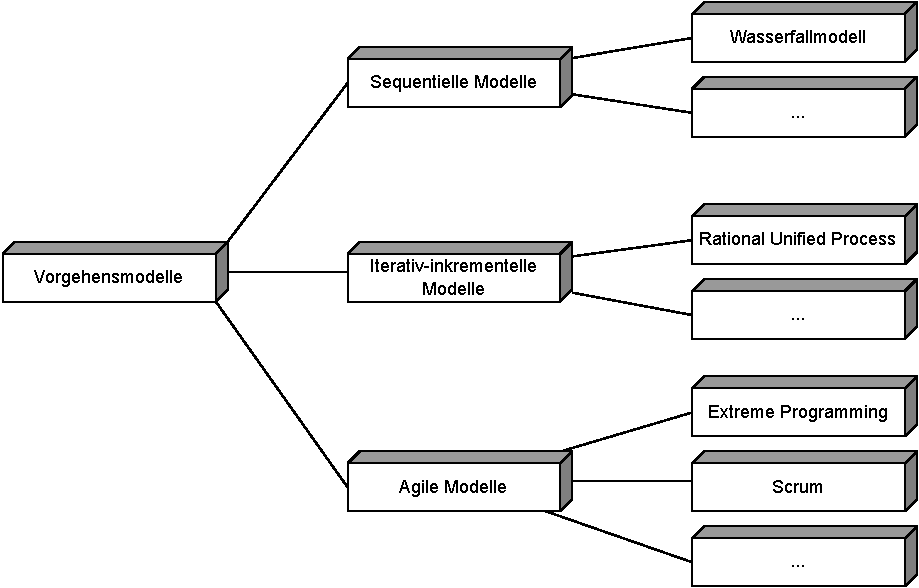
\includegraphics[scale=0.9]{Bilder/Kapitel-2/vorgehensmodelle.pdf}
	\caption{Kategorien von Vorgehensmodellen}
	\label{fig:vorgehensmodelle_komplett}
\end{figure}

Die ersten im Softwareengineering eingesetzten Vorgehensmodelle folgten einem Paradigma, das man als \textit{plangesteuert} bezeichnet. Diesem plangesteuerten Paradigma liegt die Einschätzung zugrunde, dass Softwareentwicklungsprojekte nur dann erfolgreich abgeschlossen werden können, wenn die durchzuführenden (Teil)Prozesse des Softwareengineering und ihr kausal-zeitlicher Ablauf im Vorfeld des Projekts systematisch geplant werden und spätere (Teil)Prozesse immer erst bei Vorliegen von vollständigen, qualitätsgesicherten und dokumentierten Ergebnissen vorhergehender Prozesse starten. Vorgehensmodelle, die dem plangesteuertem Paradigma folgen, gehören zur Kategorie der sogenannten \textit{sequentiellen Modelle} 
\marginline{sequentielle Modelle} 
oder Phasenmodelle. Der bekannteste Repräsentant sequentieller Modelle ist das Wasserfallmodell.

Im Unterschied zum plangesteuerten Paradigma wird im sogenannten agilen Paradigma, das seit Ende der 1990er Jahre verstärkt propagiert wird, die Einschätzung vertreten, dass ein Softwareentwicklungsprojekt nur dann erfolgreich abgeschlossen werden kann, wenn im Projektverlauf Änderungen zugelassen werden können, im Besonderen Änderungen der Anforderungen, und schon ab frühen Zeitpunkten im Projektverlauf lauffähiger (aber auch wieder änderbarer) Programmcode erzeugt wird. Vorgehensmodelle, die dem agilen Paradigma folgen, nennt man 
\marginline{agile Modelle} 
\textit{agile Modelle}. Bekannte Repräsentanten sind Extreme Programming und Scrum.

Sowohl sequentielle als auch agile Modelle werden heute im Softwareengineering eingesetzt. Konkrete Vorgehensmodelle – sowohl diejenigen, die wir in diesem Text vorstellen als auch die vielen anderen, die wir hier nicht thematisieren – passen in der Regel nicht hundertprozentig in genau eine Kategorie, da sie zusätzlich oft auch Kennzeichen anderer Kategorien aufweisen. In der Praxis gilt dies umso mehr, je stärker die Grundform eines Vorgehensmodell individuell an unternehmensspezifische Belange angepasst wird.

Wir werden in den folgenden Abschnitten sowohl allgemeiner die Kennzeichen sequentieller Modelle (Kap.~\ref{sec:Kap-2.2.1}) und agiler Modelle (Kap.~\ref{sec:Kap-2.2.3}) als auch konkrete Vorgehensmodelle als Repräsentanten dieser Kategorien von Vorgehensmodellen vorstellen. Abschnitt~\ref{sec:Kap-2.2.2} thematisiert zwischen der Vorstellung der sequentiellen und der Vorstellung der agilen Modelle eine dritte Kategorie von Vorgehensmodellen, die \textit{inkrementellen und iterativen Modelle}, 
\marginline{inkrementelle und iterative Modelle}
die in den späten 1980er und frühen 1990er Jahren erstmalig vorgestellt wurden und damit auch in ihrer Entstehungszeit zwischen den sequentiellen und den agilen Modellen liegen. Deren zugrundeliegendes Paradigma betont den Stellenwert der fachlichen Aspekte (Strukturen, Geschäftsprozesse etc.) des Einsatzgebiets des zu entwickelnden Softwareprodukts – und kritisiert damit auch die in der Regel sehr technisch orientierte Sichtweise von sequentiellen Vorgehensmodellen. Zum anderen beinhaltet es die Einschätzung, dass für erfolgreich durchzuführende Softwareentwicklungsprojekte lauffähiger Programmcode nicht erst am Ende des Projekts vorliegen darf – hier wurde die Basis für die Programmcode-Fokussierung der späteren agilen Modelle gelegt. 

\minisec{Unterscheidungsmerkmale zwischen Vorgehensmodellen}

Sequentielle, iterativ-inkrementelle (synonym: inkrementell-iterativ) und agile Vorgehensmodelle unterscheiden sich vor allem in folgenden Aspekten, die wir bei der Vorstellung der drei Kategorien in den folgenden Abschnitten jeweils im Detail betrachten werden:

\begin{enumerate}
	\item In welcher Weise werden die einzelnen (Teil)Prozesse zum Softwareentwicklungsprozess zusammengestellt?
	\item Wie wird mit neuen oder veränderten Anforderungen während der Entwicklung umgegangen?
	\item Inwieweit werden Auftraggeber und zukünftige Nutzer des zu erstellenden Softwareprodukts in die Entwicklung einbezogen?
	\item Zu welchen Zeitpunkten liegen auslieferungsfähige Produkte bzw. Teilprodukte vor?
	\item Welche Formen von Artefakten (\zb Programmcode, Dokumente, Modelle) entstehen im Laufe des Softwareentwicklungsprozesses?
\end{enumerate}


\subsection{Sequentielle Modelle}
\label{sec:Kap-2.2.1}
[\ldots]

\subsection{Inkrementelle und iterative Modelle}
\label{sec:Kap-2.2.2}
[\ldots]

\subsection{Agile Modelle}
\label{sec:Kap-2.2.3}
[\ldots]

\section{Vorgehensmodelle – Vergangenheit, Gegenwart und Zukunft}
\label{sec:Kap-2.3}
[\ldots]


%--- Kurseinheit 1 --- ENDE
%----------------------------
%--- Kurseinheit 2 --- BEGINN
%\part{Modellierung und Realwelt}
%\label{sec:KE-2}
%
%\chaptertoc % Inhaltsverzeichnis nur für diese KE
%
%\begin{refsection}
%	\input{KE2/KE2.tex}
%	
%	% Literaturverzeichnis für diese Kurseinheit
%	\newpage % auf einer neuen Seite
%	\printbibliography[heading=subbibliography]
%\end{refsection}


% Einbinden der einzelnen Kapitel
\input{KE2/KE2-Vorspann.tex}

%--- Kapitel 3
\chapter{Modelle im Softwareengineering}
\label{sec:Kap-3}

\section{Der Modellbegriff}
\label{sec:Kap-3.1}
[\ldots]

\section{objektorientierte Modellierung}
\label{sec:Kap-3.2}
[\ldots]

\subsection{Objektorientierung}
\label{sec:Kap-3.2.1}
[\ldots]

\setcounter{subsection}{4}
\setcounter{figure}{2}
\input{Kapitel-3/Kapitel-3-2-5.tex}
\input{Kapitel-3/Kapitel-3-2-5-1.tex}
[\ldots]

\section{Fallbeispiel Zoo – Ein erstes Domänenklassendiagramm}
\label{sec:Kap-3.3}
[\ldots]

%--- Kurseinheit 2 --- ENDE
%----------------------------
%--- Kurseinheit 3
%\part{Untertitel für KE3}
%\label{sec:KE-3}
%
%\chaptertoc % Inhaltsverzeichnis nur für diese KE
%
%\begin{refsection}
%	\input{KE3/KE3.tex}
%	
%	% Literaturverzeichnis für diese Kurseinheit
%	\newpage % auf einer neuen Seite
%	\printbibliography[heading=subbibliography]
%\end{refsection}

%--- Kurseinheit 3 --- ENDE
%----------------------------
%--- Kurseinheit 4 --- BEGINN
%\part{Untertitel für KE4}
%\label{sec:KE-4}
%
%\chaptertoc % Inhaltsverzeichnis nur für diese KE
%
%\begin{refsection}
%	\input{KE4/KE4.tex}
%	
%	% Literaturverzeichnis für diese Kurseinheit
%	\newpage % auf einer neuen Seite
%	\printbibliography[heading=subbibliography]
%\end{refsection}

%--- Kurseinheit 4 --- ENDE
%----------------------------
%--- Kurseinheit 5 --- BEGINN
%\part{Untertitel für KE5}
%\label{sec:KE-5}
%
%\chaptertoc % Inhaltsverzeichnis nur für diese KE
%
%\begin{refsection}
%	\input{KE5/KE5.tex}
%	
%	% Literaturverzeichnis für diese Kurseinheit
%	\newpage % auf einer neuen Seite
%	\printbibliography[heading=subbibliography]
%\end{refsection}

%--- Kurseinheit 5 --- ENDE
%----------------------------
%--- Kurseinheit 6 --- BEGINN
%\part{Untertitel für KE6}
%\label{sec:KE-6}
%
%\chaptertoc % Inhaltsverzeichnis nur für diese KE
%
%\begin{refsection}
%	\input{KE6/KE6.tex}
%	
%	% Literaturverzeichnis für diese Kurseinheit
%	\newpage % auf einer neuen Seite
%	\printbibliography[heading=subbibliography]
%\end{refsection}

%--- Kurseinheit 6 --- ENDE
%----------------------------

%\clearpage

%----------------------------
%--- Anhang --- BEGINN

%% zurück setzen, damit das Deckblatt für den Anhang korrekt erzeugt wird
%\renewcaptionname{ngerman}{\partname}{Anhang}
%\renewcommand\thepart{}
%
%% "\addparttocentry" zurück setzen, damit der Eintrag im Inhaltsverzeichnis für den Anhang passt.
%\renewcommand*{\addparttocentry}[2]{
%	\addtocentrydefault{part}{}{#2}% nur der Untertitel "Anhang" im Inhaltsverzeichnis
%}
%\appendix
%\addpart[\appendixname]{}

%%%%% Abbildungsverzeichnis
%\listoffigures

%%%%% Verzeichnis der Quellenangaben für Abbildungen
%\listoffigreferences

%%%%% Glossar ausgeben
% Default-Titel ist 'Glossar'. Will man das ändern, muss man als Option '[title=Mein Glossartitel]' angeben.
%\printglossary%[title=Mein Glossartitel]

%--- Literaturverzeichnis --- BEGINN
% Hier die Gesamt-Bibliographie ausgeben lassen.

% Tipp von hier: https://groups.google.com/g/de.comp.text.tex/c/z4_SM6hh43s
%\begin{refsection}[Kurs_1793_Literatur]	
%	\nocite{*} % alles aus Kurs_1793_Literatur.bib
	\printbibliography
%\end{refsection}
%
%--- Literaturverzeichnis --- ENDE

%%%%% Index ausgeben
%\printindex

%--- Anhang --- ENDE
%----------------------------